% -*- root: ../main.tex -*-
%!TEX root = ../main.tex
% this file is called up by main.tex
% content in this file will be fed into the main document
% vim:textwidth=80 fo=cqt

%level followed %by section, subsection


% ----------------------- paths to graphics ------------------------

% change according to folder and file names
\graphicspath{{4/figures/}}
% ----------------------- contents from here ------------------------

\todo{uncomment and edit the intro in the source code later on}

% Battery modellers face the classic  conundrum of conjuring physics-based battery
% models that remain  amenable for control applications.  Firstly, the contrasting
% nature of this modelling objective is presented. Secondly, prior attempts by the
% research community to  tackle this issue is briefly examined.  A suitable family
% of models  from the broad  category of reduced-order  models is identified  as a
% promising  candidate  for implementation  in  controls  applications. Next,  the
% drawbacks of this family of models is  discussed in detail. The state of the art
% implementation for tackling these drawbacks  is presented and their inadequacies
% are discussed.


\todo{Write the chapter. Finally come back to summarize this}


% The following efforts/trials were done (failures)
% \begin{itemize}
%     \item first attempt
%     \item second attempt
% \end{itemize}
% The following successes were achieved.
% \begin{itemize}
%     \item first attempt
%     \item second attempt
% \end{itemize}


% At the  end of this  chapter, we have a  control oriented reduced  order battery
% model amenable for use in real-time applications for SOC, SOH etc.\ estimations.


Control-Oriented  models can  be considered  synonymous with  the term  `Reduced
Order Models'. This is because the complexity of physics-based models inherently
necessitates the  use of a low  order model. In  this thesis, the two  terms are
used interchangeably.


\section{Reduced Order Models: A New Classification Scheme}\label{sec:classificationscheme}

Jokar~\etal~\cite{Jokar2016}  provide  a  comprehensive review  of  the  various
categories  of  reduced  order  physics  based  battery  models.  However,  this
work  does  not aim  to  classify  models  based on  time-vs-frequency  domains.
Fan~\etal{}~\cite{Fan2015}  conducted  a  review   of  reduced  order  modelling
methods, but  only provide an  overview of  deriving and implementing  models in
these  dual domains  without expository  analysis  of the  implications of  this
modelling choice. Unlike~\cite{Jokar2016}, this review  did not aim to provide a
classification  of various  reduced order  models, but  instead emphasises  on a
broad survey of relevant methodologies  and tools towards obtaining such models.
Hence,  neither~\cite{Jokar2016}  nor~\cite{Fan2015}  provide insight  into  the
rubrics and  implications of  the choice  of modelling in  either of  these dual
domains. Although in principle, the transformation between them follows standard
mathematical  practices,\todo{citation(s)  needed?}availability  of  models  for
final implementation  in the time domain  aids immediate uptake by  industry for
adoption  in online  \gls{bms}s. Treatment  of  reduced order  models from  this
aspect  is so  germane to  the central  hypothesis of  this chapter,\todo{can  a
simple time  domain model  do the  job?} that  the author  of this  thesis feels
compelled to undertake  a simpler classification exercise within  the context of
suitability for online implementation.


In this discussion,  various modelling methodologies and  their resultant models
are viewed  as a single  continuum and  consequently this thesis  discusses them
from such a unified perspective. Furthermore,  there is also a need to highlight
the  salient  works among  the  more  recent  advances  and extensions  to  then
prevailing  models published  since~\cite{Jokar2016} and~\cite{Fan2015}.  Hence,
the specialised  review of  reduced order modelling  literature covered  in this
section intends to supplement --- not  supplant --- the breadth of modelling art
covered between them. In particular, care  has been taken to minimize repetition
of  background art  already analysed  in these  aforementioned review  articles,
thereby striving  to report the  subset of prior  research that is  pertinent to
illustrate the  new classification scheme  introduced here. The author  does not
aim to adhere  to a chronological presentation of such  background art. Instead,
the salient  model families are  introduced in  the context of  discussing their
significance within a particular modelling technique.



Physics-based control-oriented models  can be classified as belonging  to one of
the following categories.\todo{just enumerate my classification in-line here} It
is important to distinguish between models that are derived directly in the time
domain versus  those that are  derived first in  the frequency domain  and later
converted to time domain.
\todo{enumerate all the desirable characteristics and criterion upon which
models are to be evaluated}


In  principle,  any modelling  method  that  yields a  time domain  mathematical
description of physical  phenomena that is lower in  computational complexity by
an arbitrary magnitude  than the original \gls{dfn} model can  be considered for
further investigation. In the absence of a canonical, quantitative definition of
what  constitutes a  reduced  order model,  the number  of  candidate family  of
models  to  consider  is  overwhelmingly large\todo{is  it  appropriate  to  use
such  language?}.  In  practice,  the  constraints  and  challenges  imposed  by
the  scope  of  this  work, \viz{}  suitability  for  real-time  implementation,
limits  the  choice  of  candidate  modelling  families.  For  instance,  models
relying  primarily on  classical finite  difference~\cite{Smith2006}, Galerkin's
approximation~\cite{Dao2012} or Galerkin's projection~\cite{Fan2018} methods for
transformation  and order  reduction  of  one or  more  field  variables of  the
\gls{dfn} model  are excluded. This is  done in view of  the impracticability of
implementing  such  models in  a  resource-constrained  environment such  as  an
embedded \gls{bms} controller.


Owing to  the low entry-barrier for  adoption in a real-time  controller logging
data samples  at specific time intervals,  this chapter focusses on  models that
are cast  in a  form for final  implementation in the  time domain.  This choice
implies the exclusion of those models  that are derived and implemented entirely
in the frequency domain. For the  sake of readers interested in frequency domain
methods, the discussion here briefly introduces salient literature employing the
Padé  approximation method  that serves  as  a backbone  of a  wide variety  of
frequency domain models.


\todo{can  mention  that  most  frequency domain  models  are  impedance  models
suitable for offline simulation eg An electrochemistry-based impedance model for
lithium-ion batteries}


The     transfer     function     oriented    Padé     approximation     method
for    low    order    physics-based     battery    modelling    pioneered    by
Forman~\etal{}~\cite{Forman2011a}    has   gained    widespread   adoption    in
the    areas     of    cell     design~\cite{Marcicki2013},    charge-trajectory
optimisation~\cite{Bashash2010},    controller    design~\cite{Perez2015}    and
state    estimation~\cite{Marcicki2013,Moura2012}.     Although    Prasad    and
Rahn~\cite{Prasad2013} present  an online identification  of a subset  of ageing
parameters using a Padé model and a recursive least squares algorithm, specific
implementation details such as the transformation of the Padé reduced impedance
to  discrete-time  difference  equations  was not  provided.  Padé  models  are
typically limited  to offline  applications owing  to the  aggressive trade-offs
required in the approximation order to maintain accuracy. Those models truncated
to  very low  Padé  order exhibit  poor  fidelity and  perform  no better  than
classical  equivalent circuit  models,  although recent  research attempts  have
focussed  to  mitigate  this  drawback~\cite{Yuan2017a,Yuan2017}.\todo{Should  I
discuss how they mitigated this?}


Smith~\etal{}~\cite{Smith2007}  pioneered   a  semi-hybrid   modelling  approach
to  reduced  order  modelling  and  obtained closed  form  expressions  for  all
electrochemical field variables  in the frequency domain  except for electrolyte
concentration and  potential (which were  solved separately using  the classical
finite difference discretization method). To the author's knowledge, this is the
earliest  published  instance  wherein  all  the  dynamics  of  the  full  order
model were  completely retained  in the frequency  domain. This  was facilitated
through  the use  of  transcendental  transfer functions  that  helped to  avoid
the  accuracy  degradation  brought  about  by  truncation  techniques  such  as
Padé  approximation. A  composite impedance  model was  obtained that  was then
converted  to  a  \engordnumber{12}  order state  space  model  through  residue
grouping  and truncation  techniques.  To  the knowledge  of  this author,  this
represents the first  instance in published literature  demonstrating a complete
hybrid  modelling workflow.  This model  was  capable of  predicting the  cell's
terminal voltage  within \SI{1}{\percent} of  a full-order \gls{dfn}  model. The
lumped impedance  model was  derived for  the frequency  range of  interest from
\SIrange{0}{10}{\hertz}.

This modelling effort  by Smith~\etal{} was the  first of its kind  to provide a
physics-based  battery model  for  implementation in  the classical  state-space
formulation
\begin{equation}\label{eq:statespace}
    \begin{aligned}
        \dot{x} &= Ax + Bu \\
        y &= Cx + Du
    \end{aligned}
\end{equation}
that is amenable for controller  design and  further system-level simulation
studies \eg{}  as a component in a (hybrid) electric vehicle drivetrain.


The requirement of a relatively large number of state variables (12) to describe
the system dynamics dilutes the effectiveness of state estimation algorithms. In
the classical isothermal implementation of  this model, with the cell's terminal
voltage being the only measured quantity, the observablity of the model degrades
significantly. Although Smith~\etal{} performed  an observablity analysis of the
model in  a noise-free context,  the presence  of process noise  (via unmodelled
electrochemical phenomena  and parameter uncertainties) coupled  with corruption
of measurement  values through  sensor noise in  a harsh  electrical environment
such as  in an  vehicle's drivetrain,  makes this  model unattractive  for state
estimation tasks in an online embedded application.


Several attempts have been undertaken to  improve and extend the ideas pioneered
in  Smith~\etal{}~\cite{Smith2007}.  Lee~\etal{}~addressed  a  critical  missing
aspect  of~\cite{Smith2007}, \viz{}  the derivation  of transcendental  transfer
functions  for  both the  electrolyte  concentration  and its  potential.  These
transfer  functions  were  obtained  by  using  a  Sturm-Liouville  approach  by
retaining  the first  five modes  of  the eigenfunction  expansion, as  detailed
in~\cite{Lee2012}. To the  author's best knowledge, this is  the first published
work wherein  all electrochemical  field variables of  the \gls{dfn}  model were
considered  for inclusion  in a  deterministic model  order reduction  procedure
whilst retaining the derivation entirely in the frequency domain.


Obtaining  closed form  expressions for  the electrolyte  variables achieved  in
Lee~\etal{} also has an important computational implication. With these capstone
derivations serving to completing the model description in the frequency domain,
all  electrochemical  variables of  the  \gls{dfn}  model  could now  be  solved
independently at any  desired spatial location, \eg{} at  the current collectors
and separator  interfaces. Until  this point,  the state of  the art  in reduced
order  modelling invariably  necessitated  the solution  of all  electrochemical
quantities at  multiple node locations along  the thickness of each  cell layer,
adding  to the  computational burden.  This is  a significant  deterrent to  the
adoption  of such  models if  the intended  purpose of  the model  is to  simply
predict the cell's terminal voltage.


Furthermore,  Lee~\etal{}~\cite{Lee2012a} also  devised the  \gls{dra}, a  novel
algorithm  to systematically  transform  all  transcendental transfer  functions
to  the  time domain   to  obtain  the  standard  state-space   model  given  by
\cref{eq:statespace}. The  author of  this thesis  considers the  formulation of
the  \gls{dra}  as a  breakthrough  contribution  that  has helped  in  bringing
physics-informed  time domain  models a  step  closer  to online  implementation
without   having  to   resort   to   forming  a   lumped   impedance  and   then
truncating  it  suitably.  Lee~\etal{}~\cite{Lee2014} then  extended  this  work
for  a  wider range  of  operation  across  various \gls{soc},  temperature  and
C-rates.  Although the  final  state space  model is  simple  to implement,  the
classical  \gls{dra} scheme  proposed  by Lee~\etal{}  suffers from  significant
computational bottlenecks  in forming the required  block-Hankel matrices during
the  model-derivation  phase.  A   memory-efficient  version  of  the  \gls{dra}
exploiting the  skew-symmetric structure of  these Hankel matrices  was proposed
in  Gopalakrishnan~\etal{}~\cite{Gopalakrishnan2017}  resulting  in  drastically
reduced requirements for physical memory and processing power.


In both the original  as well as the improved \gls{dra},  the computation of the
eigenfunction modal expansion of electrolyte concentration transfer function was
computationally intensive.  A less  severe disadvantage with  the transcendental
transfer  functions  associated  with  the electrolyte  concentration  was  that
their  derivation  entailed  mathematically  cumbersome  symbolic  manipulations
that  dictated  the   need  of  a  capable  \gls{cas}   package.  Although  from
a  stand-alone  viewpoint  this  requirement  does  not  seem  to  be  critical,
the  Ho-Kalman  algorithm   that  forms  a  core  component   of  the  \gls{dra}
schemes  is  steeped in  numerical  linear  algebra routines.  Furthermore,  for
facilitating  state  estimator  and  controller designs,  it  is  convenient  to
implement the resultant  state-space model in a  classical numerical computation
environment   such  as   \textsc{MATLAB}.  Taking   these  into   consideration,
Rodriguez~\etal{}~\cite{Rodriguez2017}  introduced a  simplified computation  of
the electrolyte  concentration transfer  function by  applying the  variation of
parameters  (VOP)  scheme.  With  this  final  improvement,  the  hybrid  scheme
envisaged originally by Lee~\etal{} can  be considered feature-complete with low
computational  requirements  during  both model  derivation  and  implementation
phase.


A  key  drawback  of  the  transcendental  transfer  function  approach  is  the
requirement for  linearisation at  a specific \gls{soc}.  This implies  that the
entries in  the matrices of the  state space model depends  on the linearisation
point.  In all  the  published  works employing  this  approach, these  transfer
functions were obtained  by linearising the \gls{p2d} equations  at an operating
point of  \SI{50}{\percent} \gls{soc}. The requirement  of linearisation renders
the  model usable  only  in  a narrow  range  of  \gls{soc}s. Furthermore,  this
adversely affects the usability of the model for state estimation tasks, wherein
the \gls{soc} is in fact an unknown quantity and is to be estimated.


In order  to extend  the model's  range of  validity, Lee~\etal{}~\cite{Lee2014}
proposed  a  simple model-blending  approach  by  interpolating between  several
linear models pre-computed at  different \gls{soc} and temperature combinations.
To guarantee robustness during cross-over, a  naive approach is to incorporate a
large  number  of  break-points  in  the  look-up  table.  Since  the  model  is
intended  for  online  operation,  this would  entail  significant  requirements
of  both operating  memory  and non-volatile  storage.  An alternative  approach
is  to  implement  a  fairly  coarse  break-point  table  with  a  sophisticated
changeover  mechanism. However,  this  demands careful  tuning  of the  blending
parameters  and  gain values,  an  in-depth  treatment  of  which has  not  been
detailed in Lee~\etal~\cite{Lee2014}.  Furthermore, employing these interpolated
matrices---whose  entries are  obtained  from pre-computed  matrices at  various
\gls{soc}s and temperature---for state-estimation  creates a subtle cyclic loop.
The stability  of this feedback loop  hence introduced has not  been analysed in
literature.  This  renders the  idea  of  state-estimation using  such  run-time
interpolated models  questionable.


The author  of this thesis hypothesises  that any perceivable drawbacks  such as
non-smooth changes  in \gls{soc} estimates  arising from using  blended matrices
could  be potentially  mitigated by  using  smoothing filters  and other  ad-hoc
apparatus.  However,  there  exists  no  published  work  that  discusses  these
engineering aspects. Coupled with the absence  of a theoretical analysis of loop
stability,  these  models  are  deemed  as  not  being  suitable  for  immediate
adoption  by  industry, at  least  until  these  aforementioned gaps  have  been
addressed  satisfactorily.  The non-linear  state  variable  model presented  by
Guo~\etal{}~\cite{Guo2017} aims to  address this issue by  formulating a reduced
order model in  the frequency domain by eliminating  linearisation. However, the
online solution of the model entails an complex prediction-refinement procedure,
loosely defined as implicit and explicit solution methods, for each subsystem of
the  \gls{dfn}  model.  The  formulation  of the  final  model  is  not  clearly
illustrated and  in the views of  this author, is not  easily comprehensible. In
the absence  of actual source  code, a numerical  example or pseudo-code  of the
model reduction workflow could have immensely helped with the reproducibility of
the results claimed in the work.


Physics-inspired                        equivalent                       circuit
models~\cite{Prasad2012,Prasad2014,Zhang2017,Cheng2017,Merla2018} are a class of
hybrid  models  that  have  rapidly  gained  prominence  since  the  publication
of~\cite{Jokar2016}  and~\cite{Fan2015}. The  derivation of  the relevant  model
equations  is  performed   in  the  frequency  domain.   This  frequency  domain
representation is  then converted to  a form  suitable for implementation  as an
equivalent circuit. Prasad and Rahn~\cite{Prasad2014} extended their Padé order
reduced  model first  presented  in~\cite{Prasad2013} to  convert the  impedance
model into standard  equivalent circuits. A key point to  be highlighted is that
these family of models do not necessarily strive to retain the classical Randles
structure~\cite{Randles1947}  for   their  equivalent   circuit  representation.
Instead,  the  values  of  the  electrical circuit  components  such  as  series
resistance and  equivalent capacitance  are obtained through  various mechanisms
such as \gls{eis} measurements under load.  The biggest advantage of such models
is that  they serve  as drop-in replacements  to traditional  equivalent circuit
models whilst still  retaining their origins in physical  principles rather than
on empirical curve-fitting.


\todo{can perhaps  talk about SPM converted  to equivalent circuit by  Prasad in
the IEEE conference paper}


\Cref{ch:chapter6}  briefly presents  the author's  latest work  and preliminary
results towards  obtaining a similar physics-informed  equivalent circuit model.
This  modelling  effort is  a  direct  application  of  the gains  in  computing
efficiency  through  the  application  of the  improved  \gls{dra}  reported  in
Gopalakrishnan~\etal{}~\cite{Gopalakrishnan2017},   the  detailed   coverage  of
which  is performed  in~\cref{ch:chapter3}.  This work  intends  to address  the
hitherto  unexplored  gap  in  impedance  modelling, \ie{}  the  absence  of  an
equivalent impedance  model that  accounts for  the impedance  contribution from
all  electrochemical quantities  in the  \gls{p2d} model.  This physics-informed
impedance  model can  be  extended  to fit  parameter  values  of components  in
an  equivalent circuit  model,  \eg{} by  using  a standard  Levenberg-Marquardt
non-linear least squares fitting algorithm~\cite{Levenberg1944, Marquardt1963}.


A common characteristic of  all hybrid models is the lack  of a physical meaning
to their  model parameters. This  severely limits  the insights offered  by such
models  into  electrochemical  phenomena  internal  to  the  cell.  The  biggest
attraction  of  using physics-based  models  is  the possibility  of  predicting
phenomena such as cell degradation, \eg{} through computation of the solid phase
surface concentration  and potentials  in a  vehicular application,  since their
exact  load profile  cannot be  simulated a-priori.  In this  scenario, a  model
capable of implying a direct and causal relationship between a group of physical
parameters and internal  overpotentials at various spatial  locations within the
cell serves  as a powerful  tool for  in-situ lifetime estimation  of batteries.
Although the  circuit components  of physics-informed equivalent  circuit models
and the  state-space models discussed here  trace their origins to  the original
parameters of  the \gls{dfn}  model, their  final numerical  values do  not bear
even a  semblance of this relationship.


With  goal   of  translating   physical  parameters  into   circuit  components,
Zhang~\etal{}~\cite{Zhang2017} presented a lumped equivalent circuit model based
on Padé  approximation and  model truncation. However,  the sensitivity  of the
final model  values owing to perturbation  in the original model  parameters was
not  evaluated.  Consequently, there  is  a  lack  of  clarity in  the  relative
importance  of physical  parameters  and their  influence  on circuit  component
values.


Merla~\etal{}~\cite{Merla2018} introduced  an equivalent circuit model  that can
be  parameterised by  attempting a  systematic  decoupling of  the kinetics  and
diffusion at  both electrodes  and the  electrolyte. Although  these interacting
phenomena can be complex to resolve  over all length and time-scales, acceptable
trade-offs in  accuracy was  demonstrated to be  achievable from  a system-level
simulation perspective. A  drawback of such models is that  key model parameters
such  as  solid  and  electrolyte   diffusion  coefficients  are  attributed  to
the  two electrodes  through  ad-hoc,  non-verifiable assumptions.  Furthermore,
in~\cite{Merla2018},  notable discrepancies  exist in  the values  of parameters
such as  electrolyte conductivity (obtained through  calculations from \gls{eis}
measurements) to  that typically reported  in literature. \todo{have  not talked
about SPM  inspired eq circuit model.  Is it necessary  to do so?. How  to frame
this. There are a few references that belongs to this kind}


It must be acknowledged that presently  there exists no modelling candidate that
provides  all desirable  characteristics  of  a reduced  order  model for  final
implementation in  the time domain. However,  it is strongly desirable  that the
majority  of the  final model  values  retain their  physical meaning,  yielding
system engineers and cell designers alike  with a direct and causal relationship
between  groups of  parameters and  their  influence on  the cell's  operational
performance. Since  this chapter seeks  to provide  a readily usable  model that
satisfies  all \todo{give  a number  here} criterion  for online  implementation
from,\todo{cite  figure} the  author  concludes that  at  present, the  benefits
offered by hybrid models do not decisively outweigh this drawback.


The working rubric of all time  domain reduced order models typically consist of
attempts to reformulate the original \gls{p2d}  model equations with the goal of
simplifying them.  In contrast to the  hybrid models, both the  model derivation
and  final  implementation  tasks  are  carried out  entirely  within  the  time
domain.  Whilst a  subset of  prior research  has focussed  only on  simplifying
certain aspects  of the  cell dynamics, \eg{}  solid diffusion,  other published
works  have aimed  at  providing a  simplified description  of  the time  domain
evolution of all  physical quantities of the cell. An  evaluation of the salient
literature  from both  these  approaches is  performed here.


In this discussion,  those models that entail computations with  medium or large
dense  matrices~\cite{Li2016,Xu2016,Corno2015}  or  involving concepts  such  as
fractional  order  derivatives~\cite{Sabatier2014,Sabatier2015, Li2017,  Mu2017,
Wang2017} shall not  be discussed. To this author, it  appears that the academic
community has  implicitly considered these models  to be so abstruse  that there
has not yet been a comparative  study pitting these models against the prevalent
art. Based  on published work,  it is not clear  on how such  models distinguish
themselves uniquely in the larger realm of reduced order battery.


A  few  \gls{pde}  simplification  techniques   in  the  time  domain,  such  as
Hilbert-Space  representation  and  singular   perturbation  were  presented  in
Manzie~\eta{}~\cite{Manzie2015}.  However, their  presentation lacks  expository
visual information  such as plots of  time domain evolution of the  internal and
terminal variables for dynamic load profiles. Furthermore, the authors failed to
provide a tabulated set of physical  parameters of the cell being simulated that
adversely affects the reproducibility of this  work. These methods have not seen
uptake  in academia  or  industry.  The author  of  this  thesis considers  this
presentation  to be  of a  cursory nature  and consequently,  they shall  not be
discussed here.


The  rest of  this section  discusses  several popular  families of  time domain
models. In  this section, a high-level  evaluation of their relative  merits and
weaknesses is  presented. The next section  presents a detailed analysis  of the
most promising  candidate among  these models with  the potential  to facilitate
faster adoption of physics based models in online applications. Further sections
discuss methodologies and  solutions that aim to address the  gaps identified in
this family of models. \todo{does this fit better at the end of this section}


In the \gls{dfn} model, the diffusion of Lithium in the solid phase is described
by the classical  Fick's second law~\cite{Fick1995}. In order to  solve for this
concentration  profile,  it  is  required to  discretise  every  spherical  node
(represented by the placement of a node in the axial direction) along its radial
direction (pseudo dimension). This dramatically  increases the overall number of
discretisation  nodes, adversely  impacting  the  computational efficiency.  The
impact of high node densities on  the computational requirements of the original
\gls{p2d}  model have  led researchers  to adopt  various mitigation  strategies
to  tackle  this  issue. In  contrast  to  the  pure  frequency domain  and  the
semi-hybrid/hybrid approaches discussed thus far, these attempts aim to provided
a simpler computational mesh, whilst retaining high fidelity. It should be noted
that high node  densities are mainly required near the  surface of the spherical
particles for the pseudo  \engordnumber{2} dimension. Similarly, such clustering
of nodes is desirable near the  separator and current collector interfaces along
the axial  dimension.\todo{need to define  `axial' at  the start of  the thesis}
Thus, a number  of model order reduction  strategies in the time  domain seek to
adopt  non-uniform node  spacing  towards lowering  the aforesaid  computational
issues\todo{citations needed}.


Computationally    efficient     pseudo-spectral    schemes     for    numerical
solution   of   \gls{pde}s   can be employed    by   choosing   discretisation
nodes    at    orthogonal    collocation     points    obtained    by    solving
for     the    zeros     of    certain     classes    of     polynomial    basis
functions~\cite{Ferguson1971,Trefethen2000,Boyd2001,Shizgal2015,Dutykh2016}.
Their accuracy extend beyond  the  algebraic  orders of that achievable with
classical  Finite  Difference,  Finite Element  or Finite Volume Schemes.
Northrop~\etal{}~\cite{Northrop2011} pioneered their application in battery
modelling by employing the Jacobi polynomials as underlying basis functions.
Suthar~\etal{}~\cite{Suthar2014} replaced the Jacobi polynomials with Chebyshev
polynomials to extend the applicability of the model to higher C-rates.
Bizeray~\etal{}~\cite{Bizeray2015}    provided   a detailed treatment of the
usage of Chebyshev discretisation  for   the  full   \gls{p2d} model   on  a
global  scale,  \ie{}  along  both   the  axial  and  radial directions.


The  reduced  number of  nodes  as  well as  their  clustered  placement at  the
desired  spatial  locations  enabled  by  these  discretisation  schemes  lowers
the   computational  burdens   of   simulating  a   physics-based  cell   model.
Gopalakrishnan~\etal{}~\cite{Gopalakrishnan2018} undertook a  hybrid approach by
retaining a  standard finite volume  discretisation in the axial  domain, whilst
adopting  the  Chebyshev  discretisation  only  for  the  critical  solid  phase
diffusion component in the radial direction. Albeit in time domain, the standard
\gls{p2d} equations, their boundary conditions and corresponding field variables
are  mathematically transformed  to the  Chebyshev space  within which  they are
solved.  The details  of this  transformation is  presented in  \cref{sec:hybrid
fv-spectral}  in  \cref{ch:chapter2}  for the  solid-phase  diffusion  equation.
Finally,  these solved  quantities  are  converted back  to  the physical  space
through  a corresponding  inverse transformation.  Although this  bi-directional
transformation is  algebraic in nature,  the requirement of running  a spatially
resolved model coupled with  such variable-transformation overheads render these
class  of  models unsuitable  for  online  implementation. The  contribution  of
Lee~\etal{}, \ie{} the  ability to solve for any electrochemical  variable at an
arbitrary  spatial  location by  completely  eliminating  the need  for  spatial
discretisation assumes particular significance in this context.


In all  non-uniform discretisation schemes  discussed here, the  implications of
using  a non-adaptive  support mesh  obtained by  the placement  of nodes  whose
locations are optimised a-priori, must be considered carefully. For instance, in
the long-term  usage of the cell  \eg{} in an electric  vehicle application, the
reaction front drifts  from separator back towards the  current collectors. This
is  due to  the exhaustion  of  Lithium at  the  surface of  particles near  the
separator  interfaces.  In  this  scenario,  the  solutions  produced  by  these
models could  be worse than  simpler models with uniform  mesh-density. Although
adaptive meshing strategies can be  employed for desktop simulation with minimal
effort,  it remains  to  be seen  if  this  can be  deployed  successfully in  a
resource-constrained environment  such as an embedded  \gls{bms} controller, and
hence warrants  further research.\todo{does  this fit  better in  the conclusion
chapter?}


The  computational  bottlenecks arising  due  to  discretisation in  the  radial
direction  have  motivated  researchers   to  explore  mesh-free  approaches  to
solve for  solid phase  concentrations. Subramanian~\etal~\cite{Subramanian2004}
pioneered  the concept  of employing  polynomial approximations  of the  Fickian
diffusion equation to solve for Lithium concentrations in the porous electrodes.
Here,  the solid-phase  surface  concentrations was  expressed  as a  correction
term  applied  to their  average  concentrations  which  was described  using  a
second degree polynomial. In  a follow-on study~\cite{Subramanian2005}, the same
authors  presented a  solution using  higher order  polynomials and  performed a
dimensionless analysis of their  proposed reformulation. In the \engordnumber{2}
and  \engordnumber{3}  order  solutions,  the polynomial  equation  for  surface
concentration was  accompanied by a  corresponding \gls{ode} for  describing the
temporal  evolution of  average concentration,  thereby leading  to a  system of
\gls{dae}s. Furthermore, Subramanian~\etal{}~\cite{Subramanian2007} demonstrated
the  application  of  polynomial  approximation  of  solid  phase  diffusion  by
simulating a complete \gls{dfn} model.


Using polynomial  approximation for the  solid phase concentration results  in a
drastic reduction  in the number  of \gls{dae}s needed  to solve the  full model
since now discretisation  needs to be performed only along  the axial direction.
The  polynomial  approximation  solution  applied   to  solve  for  the  surface
concentration in  the solid phase can  hence be viewed as  a dimension reduction
approach, as  it removes  the model's  dependence in  the radial  direction. The
textbook by  Carslaw and  Jaeger~\cite{Carslaw1947} details the  derivations for
obtaining the  standard analytical solution  to Fick's  law of diffusion  in the
context of heat conduction in solids. Liu~\cite{Liu2006} derived this analytical
solution for the  Lithium intercalation process in the solid  phase, taking into
account  the  idiosyncrasies  of porous  electrodes\todo{explain  about  Olcer's
pseudo-steady state  stuff}. However, this  expression involves an  infinite sum
expansion of eigen  modes. Guo and White~\cite{Guo2012}  formulate an expression
for  truncated approximation  of this  solution  to arbitrary  number of  terms.
Furthermore, they  demonstrated the validity  of this solution by  comparing the
analytical solution  truncated to the  first 5 terms  with that obtained  from a
classical finite  element solution. However, this  truncated analytical solution
involves exponential and trigonometric terms  and is non-trivial to implement on
\gls{bms} chips lacking support for floating point computations. Moreover, there
has been no extensive study comparing  the analytical solution to the polynomial
approach. Consequently, this  approach has not yet  gained widespread popularity
in the inherent elimination of the radial dimension embedded as a core aspect of
the  cell-level model  order reduction  approaches discussed  here.\todo{another
method of solving  this diffusion is the integral method  analysis used by Tanim
etal. Should  I mention that?.  There is also  a comprehensive review  by Romero
etal. Furthermore, there is a specific review by Zhang and White}

\todo{In the words of  Zhang and White, ``The usage of the  PSS method is mainly
affected by the num- ber of summation  terms included. If no summation terms are
used, the  method degrades to  the low  order polynomial method.  Increasing the
number of summation terms improves the accu- racy of the method, mostly at short
times. Our simulation shows that PSS method with two or three summation terms is
able to  provide accurate results  under a  wide range of  operating conditions.
More summation  terms require solving  more differ- ential equations  (Eq. (9b))
and could pose numerical difficulties because of the exponential terms.''}

\todo{There are way too many models that use the proper orthogonal decomposition
technique. Should I review these?}


The computational  speed-up facilitated  by using polynomial  approximations for
the  solid  phase diffusion  has  motivated  other  researchers to  extend  this
approach for representing  all other electrochemical variables  of the \gls{dfn}
model. Deng~\etal{}~\cite{Deng2018} presented a  polynomial approximation of the
full \gls{p2d}  model, whose notable  contribution is in providing  a polynomial
approximation for  the molar flux  density along the  thickness of the  cell.
% To the  author's knowledge,  this  is  the first  attempt  to  provide a  spatially dependent  simplified  approximation  of  the  interfacial  flux  density.
This presents a well-balanced choice between the  need to use the strongly
non-linear Butler-Volmer kinetics or having to resort to a lumped representation
of average kinetic behaviour.  Hence, this  model is particularly  suited to
reduced order modelling  of  cells  with  medium  electrode  thicknesses wherein
the  lumped representation of flux density is not applicable.

% In this work, the issue of equation deficiency in polynomial representation of
% the  electrolyte  concentration  was  avoided by  using  a  simpler  quadratic
% polynomial within the porous electrode regions.


One  serious  drawback in  Deng~\etal{}~\cite{Deng2018}  is  the use  of  Finite
Difference approximation  for computing the  spatial gradient of  the \gls{ocp}.
This  adversely  affects  computational  performance and  is  not  suitable  for
online implementation.  The author's efforts  to replace this  finite difference
calculation of  the gradient  with an  analytical framework  based on  the chain
rule  of calculus  is  currently in  preliminary stages  of  development and  is
presented in~\cref{ch:chapter6}. Unless a proven solution for such computational
challenges is  made available,  it is  worthwhile to  continue to  explore other
available physics-based models to identify  the most apropos first candidate for
adoption in real-time \gls{bms} environments.


Farag~\etal{}~\cite{Farag2017}  proposed  a  piecewise linear  approximation  of
all  governing  equations  of  the  electrochemical  model.  Given  that  linear
approximations are simplistic  in nature, the authors acknowledged  that a naive
implementation shall  result in a  crude approximation of the  model's dynamics.
Hence,  an optimal  knot-placement  scheme  was proposed  and  solved through  a
genetic  algorithm. Since  this Computationally  intensive step  occurs offline,
this does not adversely affect the real-time performance of the model. The final
model is  implemented using standard  state-space matrices. However,  this model
also suffers  from the  drawbacks of  the hybrid  modelling approaches,  \ie{} a
complete lack  of physical interpretation of  its parameters. As with  any other
model involving \gls{soc} based linearisation points, the stability of the model
to uncertainties in physical parameters  is questionable. A detailed sensitivity
analysis of the  knot placement scheme's output to such  parametric variation is
to  be performed,  establishing  confidence in  the  model's robustness,  before
such  piecewise  linear approaches  can  gain  widespread acceptance  in  online
applications.


\todo{Tikz  picture  here, showing  a  nice  layout of  various  models
according to the new classification scheme.}

\todo{spider  drawing   on  5  counts---  simplicity,   parametrisation,  online
implementation, state estimation, physical insight}


Referring  to   \todo{spider  figure   reference},  it   is  evident   that  all
physics-based  reduced  order  models   presented  thus  far  entails  extensive
parametrisation efforts  \todo{at the  end, count  and substitute  the canonical
number of  parameters here} to render  them useful for a  practical application.
The  difficulties associated  with such  parametrisation, coupled  with inherent
uncertainties  in  the obtained  parameter  values  act  as a  strong  deterrent
to  stakeholders  outside academia  to  adopt  physics-based models  for  online
implementation  in  a   \gls{bms}.  This  motivates  the  need   for  a  simpler
physics-based models and a family of such models is introduced next.


Haran~\etal{}~\cite{Haran1998}  proposed a  highly simplified  representation of
porous  electrodes for  the metal  hydride cell  chemistry. In  this work,  each
porous electrode  was represented as  a single spherical particle.  This concept
was adopted for Lithium ion batteries  by Ning and Popov~\cite{Ning2004} and has
since  become highly  popular. Models  employing this  lumped representation  of
electrodes  are referred  to as  \gls{spm}s. These  models have  three advantages.
Since  they involve  only  a  subset of  parameters  of  the original  \gls{dfn}
model, most  of them being  geometric quantities  that can be  directly measured
without  extensive chemical  or  electrical testing,  \gls{spm}s  are easier  to
parameterise than other physics-based reduced order model. Furthermore, they are
computationally cheap, especially when coupled with the polynomial approximation
for solving the solid diffusion equation for each electrode. Finally, all model
parameters in the \gls{spm} retain their physical character, aiding in a direct
and intuitive understanding of physical parameters on the cell's operation.


Prima Facie, based  on a preliminary comparison of the  strengths and weaknesses
of  the  modelling  families  in  the  literature  considered,  the  overarching
simplicity of  \gls{spm}s and their  immediate potential  to bring the  power of
physics-based prediction  to an embedded  environment is a strong  motivation to
pursue their in-depth exploration. The  equations describing the single particle
model  is introduced  in  \ldots. An  in-depth analysis  of  their drawbacks  is
presented in \ldots. Various attempts to  fix this issue is presented in \ldots.
The  electrolyte  concentration and  potential  fixes  is presented  in  \ldots.
Finally, results and discussion. \todo{REWRITE after finishing up everything}


% \todo{Where does this  paragraph go? End of this section/end  of chapter or even
% last  chapter?} The  identification of  individual parameters  of the  \gls{dfn}
% model  remains a  key  area in  battery modelling  that  remains only  partially
% explored. Nevertheless, this effort is critical  to ensure rapid adoption of any
% physics-based model and  sophisticated control algorithms. The state  of the art
% in this area, the challenges involved  and current efforts in this direction are
% explored in~\cref{ch:chapter6}.  Although sensitivity analysis of  the \gls{dfn}
% parameters has been performed in  literature, \todo{citation here} the extent to
% which  parameter uncertainties  influence the  numerical  values in  the $A,  B,
% C$  and  $D$  matrices  of~\Cref{eq:statespace} has  not  yet  been  attempted.
% In  continuation of  this  research  aspect, the  order  of  magnitude shift  in
% eigen/singular values of  the relevant system matrix also need  to be quantified
% to  enable an  informed  choice about  stability of  such  models for  real-time
% implementations.


\section{The Single Particle Model}

% As  discussed in  \cref{sec:classificationscheme},\todo{may need  to cross-ref
% the relevant subsection}


Reducing  the   number  of   computational  dimensions   in  a   physical  model
helps  in  formulating  their  low order  approximations,  thereby  facilitating
fast   computations.   The  \gls{spm},   originally   used   in  modelling   the
Metal-Hydride    chemistry~\cite{Haran1998}   and    later   on    adapted   for
Li-ion   cells~\cite{Ning2004},  represents   the  canonical   apogee  of   such
dimension-reduction strategies.


During the initial  years following its inception, the formulation  of the basic
\gls{spm} has  been discussed  extensively within  application-specific contexts
such  as  \gls{soc}  estimation~\cite{Santhanagopalan2006a,Santhanagopalan2008},
parameter   estimation~\cite{Santhanagopalan2007},   life   cycle   and   ageing
predictions~\cite{Santhanagopalan2008a,Safari2009}.   There   have   also   been
detailed    stand-alone    presentations    of    various    facets    of    the
basic   \gls{spm},   such   as    its   inherent   assumptions   and   governing
equations~\cite{Santhanagopalan2006,Chaturvedi2010}.    The   basic    \gls{spm}
suffers    from    certain    major     limitations    which    are    discussed
in~\cref{subsec:basicspmlimitations}. Since the turn  of the decade, researchers
have attempted to tackle many of these  issues and such efforts are discussed in
\cref{sec:electrolyteinclusion}.


A  survey of  the  most recent  literature  in all  \gls{spm}  family of  models
reveals a  diminishing rate of  advancement in quantifiable improvements  to the
underlying  plant model.  This  nearly-static  trend can  be  attributed to  the
general consensus  within the research  community that  these models may  be too
simplistic and not  of suitable accuracy to warrant further  studies. Other than
a  small  minority  of  papers  that  propose  core  modelling  improvements  to
tackle  their modelling  inaccuracies  or  add new  enhancements~\cite{Li2017a},
latest  work in  this  family of  models predominantly  pertains  to the  topics
of    state   estimation~\cite{Chaochun2018,Lin2017,Tran2017,Moura2017,Zou2016},
optimal    charging~\cite{Perez2015},    cycling    performance~\cite{Maia2017},
conversion           to            equivalent           circuits~\cite{Li2017b},
parametrisation~\cite{Li2018,Rajabloo2017,Bizeray2017,Namor2017}   and  observer
design for joint  state--parameter estimation~\cite{Ascencio2016}. The \gls{spm}
approach was  also extended to  the case of  composite electrodes, leading  to a
state  estimator design  after basic  observablity analysis~\cite{Bartlett2015}.
Owing to their simplicity, this author believes that \gls{spm}s hold the highest
potential to bring a physics based  model to embedded \gls{bms}s. With this goal
in view,  this thesis seeks  to resurrect interest  in this field  by addressing
this paucity  in fundamental model  improvements. A proposed enhancement  to the
basic \gls{spm} is the main contribution  of this chapter and shall be discussed
in~\cref{sec:newelectrolytemodel}.


In  order  to establish  a  context  for discussing  the  author's  work, it  is
imperative to provide  a holistic presentation of the  basic \gls{spm} modelling
art. The conventional \gls{spm} is the simplest of all time domain physics-based
models and  the rest  of this  section provides an  expository treatment  of its
rubrics.


\subsection{Model Development --- Geometry}

\begin{figure}[h]
    \centering
    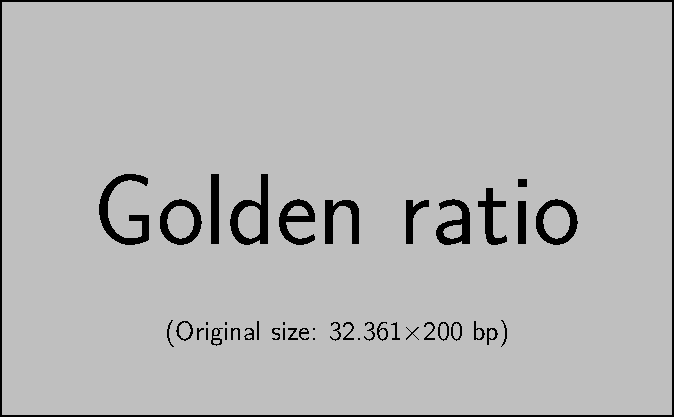
\includegraphics[width=\textwidth]{placeholder_images/example-image-golden.pdf}
    \caption[Schematic illustration depicting geometrical origins of the \gls{spm}]
    {Schematic illustration depicting the geometrical origins of the \gls{spm}. The \gls{spm} is obtained through a degenerate spatial discretisation of one electrochemical layer within a typical Li-ion pouch cell. The axial direction along the cell's thickness is denoted by $x(t)$, whilst the pseudo-dimension along the radial depth of each electrode particle is denoted by $r(t)$. In the basic \gls{spm}, the active material of each porous electrode is represented by one representative spherical particle, thus entirely eliminating the spatial dimension along the axial direction.}
    \label{fig:sandwichtospm}
\end{figure}


\Cref{fig:sandwichtospm}  shows the  arrangement  of  one electrochemical  layer
within a  typical Li-ion pouch cell.  A description of the  working principle of
the  cell was  presented in~\cref{ch:chapter1}  and  is not  repeated here.  The
\gls{spm}, as the name suggests,  models the electrochemical phenomena along the
thickness  $l_j$, \jinnegpos{}  of  each porous  electrode  by a  representative
spherical particle.  Thus the two  distinct solid-phase porous materials  of the
cell, \ie{} the  negative and positive electrodes, are idealised  as two spheres
of radii $r_\text{neg}$ and $r_\text{pos}$ respectively.


In  this  reformulated  arrangement,  the  spatial  dimension  along  the  axial
thickness  of  each  electrode  degenerates   to  a  single  point.  Hence,  the
concentration of Lithium within each electrode $c_{\text{s}_j}$, \jinnegpos{} is
only a  function of the radial  position $r_j$, \jinnegpos{} along  the depth of
their  representative  spherical  particle,  and time,  $t$.  The  surface  area
of  each representative  sphere  is  scaled appropriately,  such  that they  are
equivalent  to the  active area  of  the corresponding  porous electrodes.  Thus
the  \gls{spm} accounts  for  the  reduced volume-fraction  arising  due to  the
microporous structure of  the solid-phase. However, the storage  capacity of the
representative  particles  match  that  of  the  corresponding  electrodes.  The
overarching  assumption  of  the  \gls{spm} modelling  philosophy  is  that  the
electrochemical performance of these representative electrodes are sufficient to
model the behaviour of the cell at its terminals. The \gls{spm} thus employs the
coarsest possible spatial  discretisation of the cell's thickness  with the goal
of minimising computational burden.


\subsection{Model Development --- Scope and Assumptions}

Having established the geometrical representation of the model, it is imperative
to establish its  aims and scope. This section discusses  the subset of physical
phenomena that can captured by the model and enumerates the inherent assumptions
in  model derivation.The  validity of  these  assumptions and  their effects  is
discussed  in~\cref{subsec:basicspmlimitations}.  As  a  broad  outline  of  the
\gls{spm}s scope,  the model  attributes the cell  polarisation to  two dominant
physics,  \viz{} reaction  kinetics and  solid-phase transport  phenomena, \ie{}
diffusion dynamics.


The  \gls{spm}  assumes that  charge  transfer  happens throughout  the  surface
of  each  representative  spherical  particle where  intercalation  occurs.  The
electronic  conductivity of  the solid-phase  is assumed  to be  high enough  to
ignore the  spatial distribution of  charge, \ie{} the local  volumetric current
density is assumed  to be uniform along the thickness  of each porous electrode.
This assumption is  motivated by the early calculations performed  by Newman and
Tobias~\cite{Newman1962} in their stand-alone  analysis of current distributions
in porous electrodes, wherein a volume-averaged molar flux is deemed sufficient.
This uniform current density assumption implies that all of the particles in the
electrode active material are in parallel.


In the  \gls{spm}, solid-phase  diffusion dynamics are  solved by  assuming this
averaged electrochemical  reaction rate.  In the simulation  study by  Smith and
Wang~\cite{Smith2006b},  it  is  reported  that, soon  after  the  beginning  of
discharge, solid-phase concentration and ionic flux become nearly independent of
spatial position, and  Lithium diffusion in solid particles may  be driven by an
averaged molar flux at the surface.


Based  on the  discussion thus  far, it  is clear  that the  \gls{spm} does  not
attempt  to model  all physical  processes within  the cell.  The model  assumes
instantaneous  charge transport  from one  electrode  to the  other through  the
solution phase.  This implies that  electrolytic diffusion is  sufficiently fast
(relative to  diffusion in the solid  phase). Thus, mass transport  phenomena in
the  electrolyte  are  not  considered.


During the  operation of the  cell, the  \gls{spm} assumes that  the electrolyte
concentration  $c_\text{e}$ remains  constant at  its equilibrium  initial value
$c_{\text{e},0}$ throughout  the cell thickness. Neglecting  local concentration
gradients  in the  solution phase,  together  with ignoring  its mass  transport
phenomena implies that  the current in the electrolyte does  not vary over space
and time. Hence,  in the conventional \gls{spm} there is  no contribution of the
solution  phase  to internal  overpotentials  and  electroyte dynamics  have  no
influence on the cell's terminal voltage.


Finally,  the  \gls{spm}  ignores  any   variations  in  material  porosity  and
ionic-flow tortuosity  along the axial  direction of the cell.  This facilitates
the  usage of  a constant  effective diffusion  coefficient for  the electrolyte
phase. Furthermore,  the solid-phase diffusion  and kinetic parameters  are held
constant. Thermal effects are assumed to be negligible and no degradation
effects are attempted to be modelled.


These simplifying  assumptions are  made so  as to enable  the formulation  of a
physics-based model without incurring a  heavy computational cost. The impact of
these  assumptions shall  be  examined in~\cref{subsec:basicspmlimitations}  and
later  sections presents  research that  strives  to straddle  the fine  balance
between model sophistication and computational complexity.


\subsection{Model Development --- Chemistry}

This section  provides a  brief overview of  the essential  chemistry principles
that helps to provide a background context for the governing equations presented
in~\cref{subsec:basicspmgoverningeqns}.


In  a Li-ion  cell,  the  positive electrode  consists  of  porous particles  of
Lithium--Transition Metal Oxide (MO) compounds. The negative electrode typically
employs  some  variant  of  microporous  graphite.  The  porous  nature  of  the
electrodes  provide interstitial  sites  which act  as  intercalation spots  for
Lithium shuttling  between the two  electrodes. The electrolyte,  whose dynamics
are ignored  in the \gls{spm},  helps in the  conduction of \ce{Li^+}  ions. The
separator membrane allows the passage of  these ions between the two electrodes,
but prevents internal short-circuit  by inhibiting electronic conduction through
it. The current collectors facilitate  passage of electrons generated during the
charge transfer reaction  at particle surface to the external  circuit. With the
help of~\cref{fig:chargetransferprocess}  the steps involved in  this process is
detailed next.

\begin{figure}[h]
    \centering
    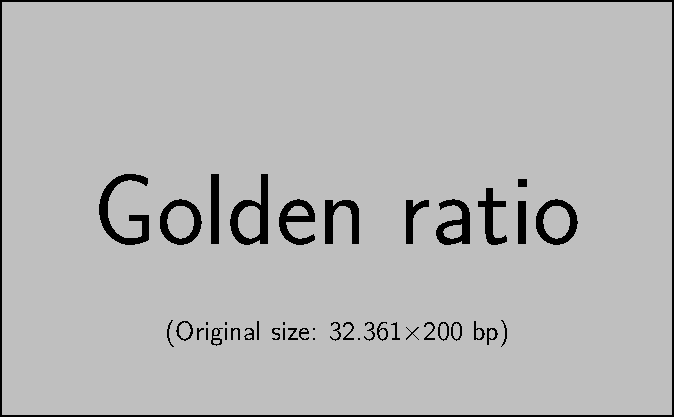
\includegraphics[width=0.5\textwidth]{placeholder_images/example-image-golden.pdf}
    \caption
    {Simplified representation of charge-transfer process and illustration of
    basic working mechanism of a Li-ion cell}
    \label{fig:chargetransferprocess}
\end{figure}

At fully charged  condition, majority of Lithium in the  system is packed within
the negative electrode microstructure. During discharge, \ce{Li^0} atoms diffuse
out  of  deep  interstitial  sites  towards the  surface  of  the  particles  in
the  negative electrode.  At  the surface  (electrode-electrolyte interface),  a
charge-transfer process takes place according to Butler-Volmer kinetics, leading
to  the formation  of \ce{Li^+}  ions and  electrons. The  electrons are  passed
to  the external  circuit  through  \ce{Cu} current  collectors  onto which  the
conductive matrix  composed of  the negative electrode  material and  binders is
coated. The  \ce{Li^+} ions travel  through the electrolyte phase,  crossing the
separator membrane  to the positive  electrode where they encounter  an electron
influx from the external circuit. A  charge transfer reaction takes place at the
surface of the positive electrode particles, leading to the formation of neutral
\ce{Li^0} atoms that diffuse into the positive electrode microstructure.

During  the   charging  process,  the   reverse  phenomena  occur.   Lithium  is
de-intercalated  from  the  positive  electrode and  a  similar  charge-transfer
occurs  at  the surface,  leading  to  the  formation  of \ce{Li^+}  ions  which
reach  the  negative  electrode  by   passing  through  the  separator.  At  the
surface  of  the  negative  electrode particles,  these  ions  absorb  electrons
from  the  external circuit,  leading  to  the  formation of  neutral  \ce{Li^0}
that   diffuses  into   interior   vacant  spaces   in   the  layered   graphite
electrode. The  charge-transfer mechanism  and sequence  of events  are depicted
in~\cref{fig:chargetransferprocess}.

\begin{align}
    \ce{Li_${x}$ C &<=> C + x Li + xe^-} \\
\end{align}

\ce{Li_x C <=> C + x Li + xe^-}

\ce{CO2 + C <=> 2 CO}

Equations summarise the reactions during the charging and discharging process at
the surfaces of both electrode materials. Assuming no loss of cycleable Lithium
due to parasitic side reactions or other mechanisms, the entire process is
reversible.


The potential of each electrode is  dependent upon the extent of its lithiation.
An empirical relationship of each electrode's potential as a function of its
stoichiometry can be obtained, and is dependent upon the specific design and
material properties of each active material under consideration. Finally, the
\gls{ocv} of the cell is obtained by subtracting the negative electrode
potential from its positive electrode counterpart.

\subsection{Limitations and Drawbacks}\label{subsec:basicspmlimitations}

The modelling foundations of the \gls{spm} have been


\section{Electrolyte Inclusion}\label{sec:electrolyteinclusion}

Rahimian~\etal{}~\cite{KhaleghiRahimian2013} discuss  the usage of  a polynomial
approximation  for   electrolyte  concentration  and  potentials.   However,  no
restriction was imposed on the order  of the polynomials chosen to represent the
electrolyte concentration within  each porous electrode region.  In the standard
\gls{dfn} model, the  number of equations and  corresponding boundary conditions
describing electrolyte charge and mass transport within the cell is insufficient
to uniquely solve for all  unknown coefficients of the polynomial approximation.
The  challenges  posed  due  to  this equation  deficiency  shall  be  discussed
in~\cref{temp:eqndeficiency}. Although  the original  \gls{spm} did  not involve
solving  for  the  electrolyte  concentrations  or  potentials,  The  polynomial
approximation of the single


Rahimian~\etal{} adopted  a cubic  polynomial for approximating  the electrolyte
concentration within  the porous electrodes.  To overcome the issue  of equation
deficiency, they adapted a scheme wherein one additional spatial location in the
interior  of  each  electrode  was  used. The  coefficients  of  the  polynomial
approximation  were then  obtained  by iteratively  solving  a relatively  large
coupled  system of  algebraic equations,  embedding within  them the  additional
equations evaluated at  the interior point. An additional  complicating issue is
the specific positioning of this  additional interior point. An online numerical
optimisation  was performed  to obtain  the optimal  placement of  this interior
node. Although it serves as a proof of concept towards implementing higher order
polynomial approximations,  the author of this  thesis deems this method  as too
complex for online implementations.

\section{New Electrolyte Model}\label{sec:newelectrolytemodel}



\subsection{equation deficiency \dots}\label{temp:eqndeficiency}

% \begin{figure}[htb]
% \begin{algorithmic}[1]

% \Procedure{SUM}{ $\{x\}$}

% \State $y\gets0$
% \For{$i \gets 1 : N^{x}$} \Comment{Time series $\{x\}$ has length $N^{x}$}
%    \State $y\gets y+x(i)$ \Comment{Summing up.}
% \EndFor

% \State \textbf{return}  $y$
% \EndProcedure
% \end{algorithmic}
% \caption[Implementation of a algorithm for calculating a sum.]{Implementation of a algorithm for calculating a sum.}
% \label{fig:algorithm1}
% \end{figure}




% ---------------------------------------------------------------------------
%: ----------------------- end of thesis sub-document ------------------------
% ---------------------------------------------------------------------------


